\section{Trigger rate}
\label{sec:trigrate}

Although the proposed algorithm rescues the y-resolution, the presence of the extra roads in the $U$,$V$ planes greatly increases the number of triggers found per BC. Under high background conditions, the MMTP cannot be a standalone trigger. With 2.2m (0.5m) long strips and an implementation region of 136 (96) roads, we have an average of 0.02 (0.004) triggers per BC with 40 kHz/strip of background. This averages to be about 0.3 triggers per BC in the entire NSW. 
\par To meet latency and resource requirements, the number of triggers that need to be processed must be as small as possible. Processing 1-2 triggers per BC is easily managed by the MMTP. However, the number of triggers per BC spikes when a muon passes through. Without any background hits, each hit can satisfy up one or two $X$, $U$, or $V$ roads with the neighboring-road effect, and therefore we can can make up to 6 triggers per BC. When the background hits are added, this number can go up to 15 triggers per BC, as shown in Fig. \ref{fig:ntrig}. Note that the distribution of the number of triggers in a given BC depends on which BC you are looking at. Fig. \ref{fig:ntrig} shows the distribution of the number of triggers for \textit{one} BC. We look at the BC in which the first real muon hit has been in the MMTP buffer for 8 BCs. This is the BC with the highest average number of triggers.
\par It is unclear how to process all of these triggers in a timely fashion in the FPGA. This is to be determined.
\begin{figure}[!htpb]
  \begin{center}
    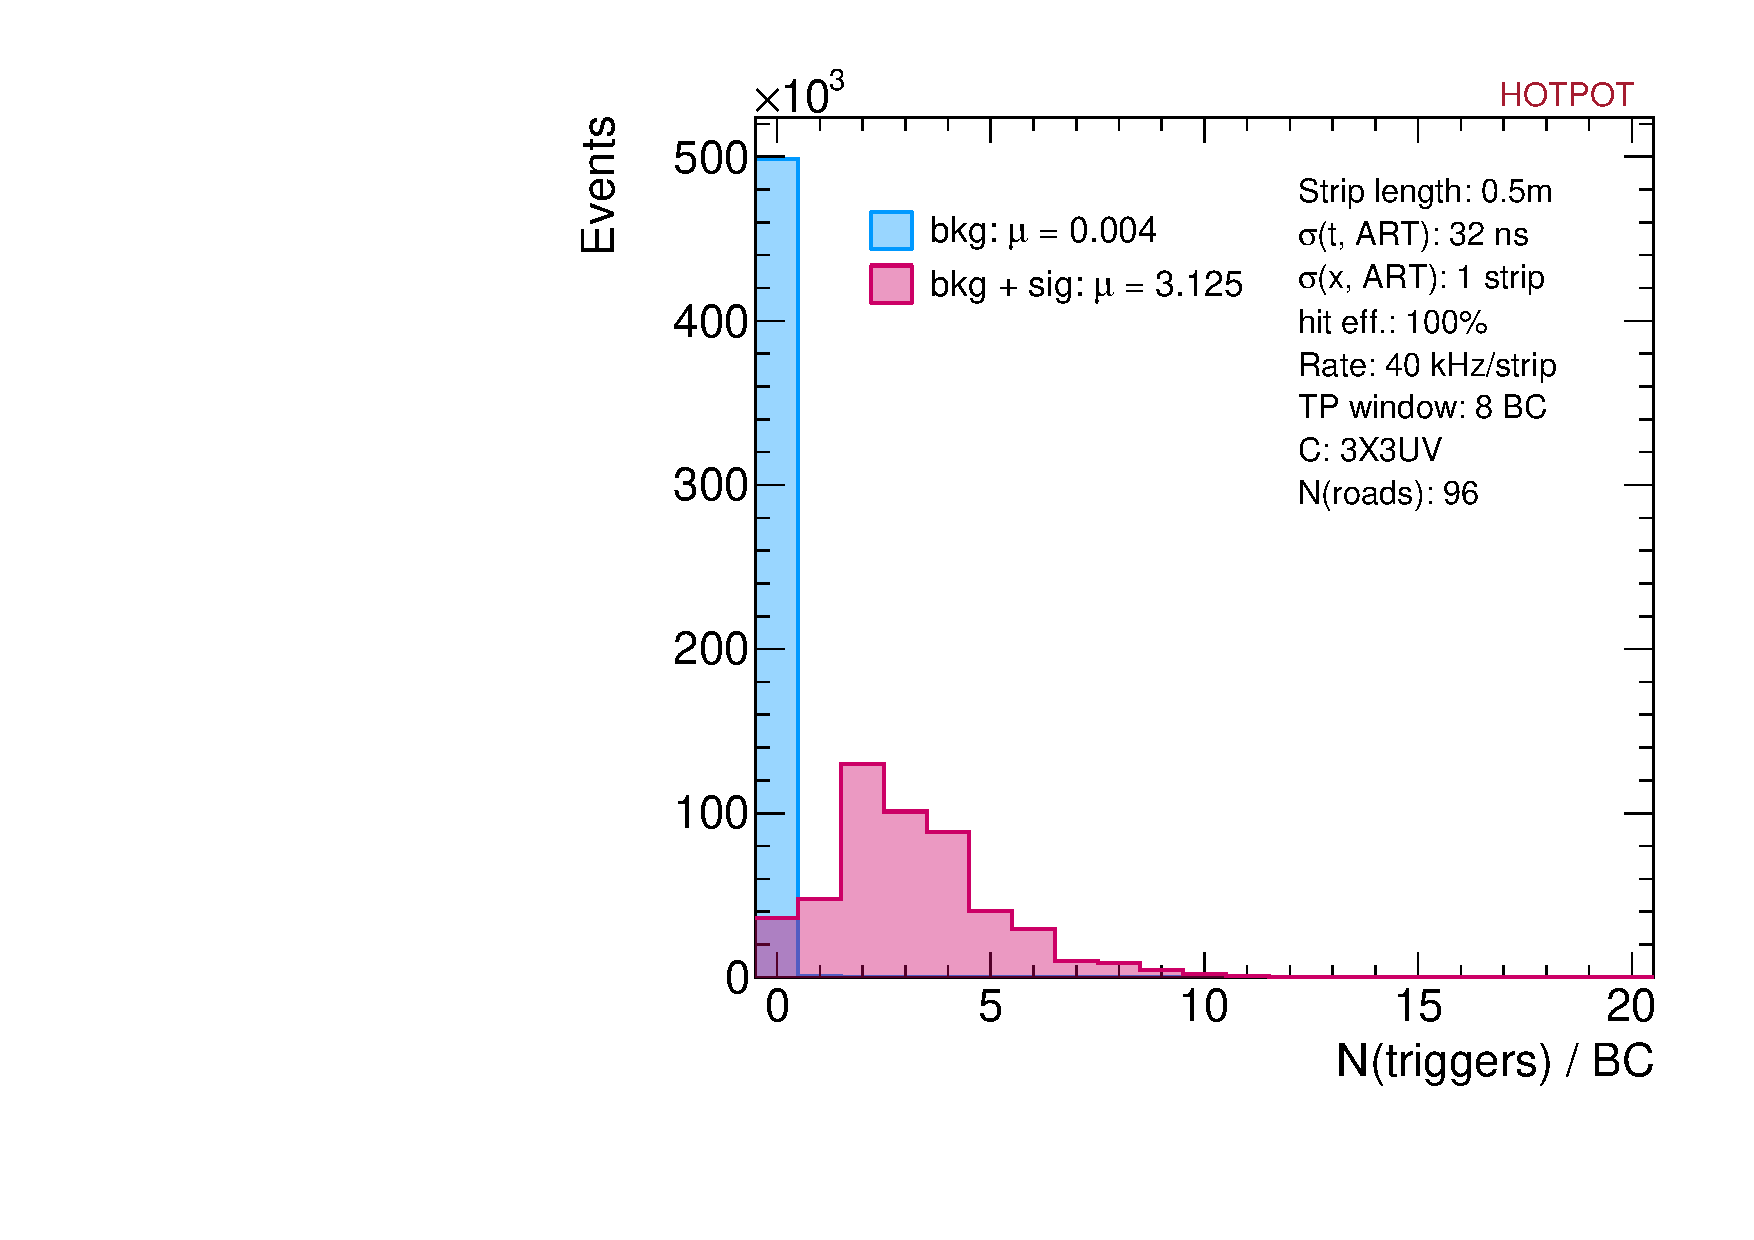
\includegraphics[width=0.48\textwidth]{figures/r96_ntrig_BC7.pdf}
    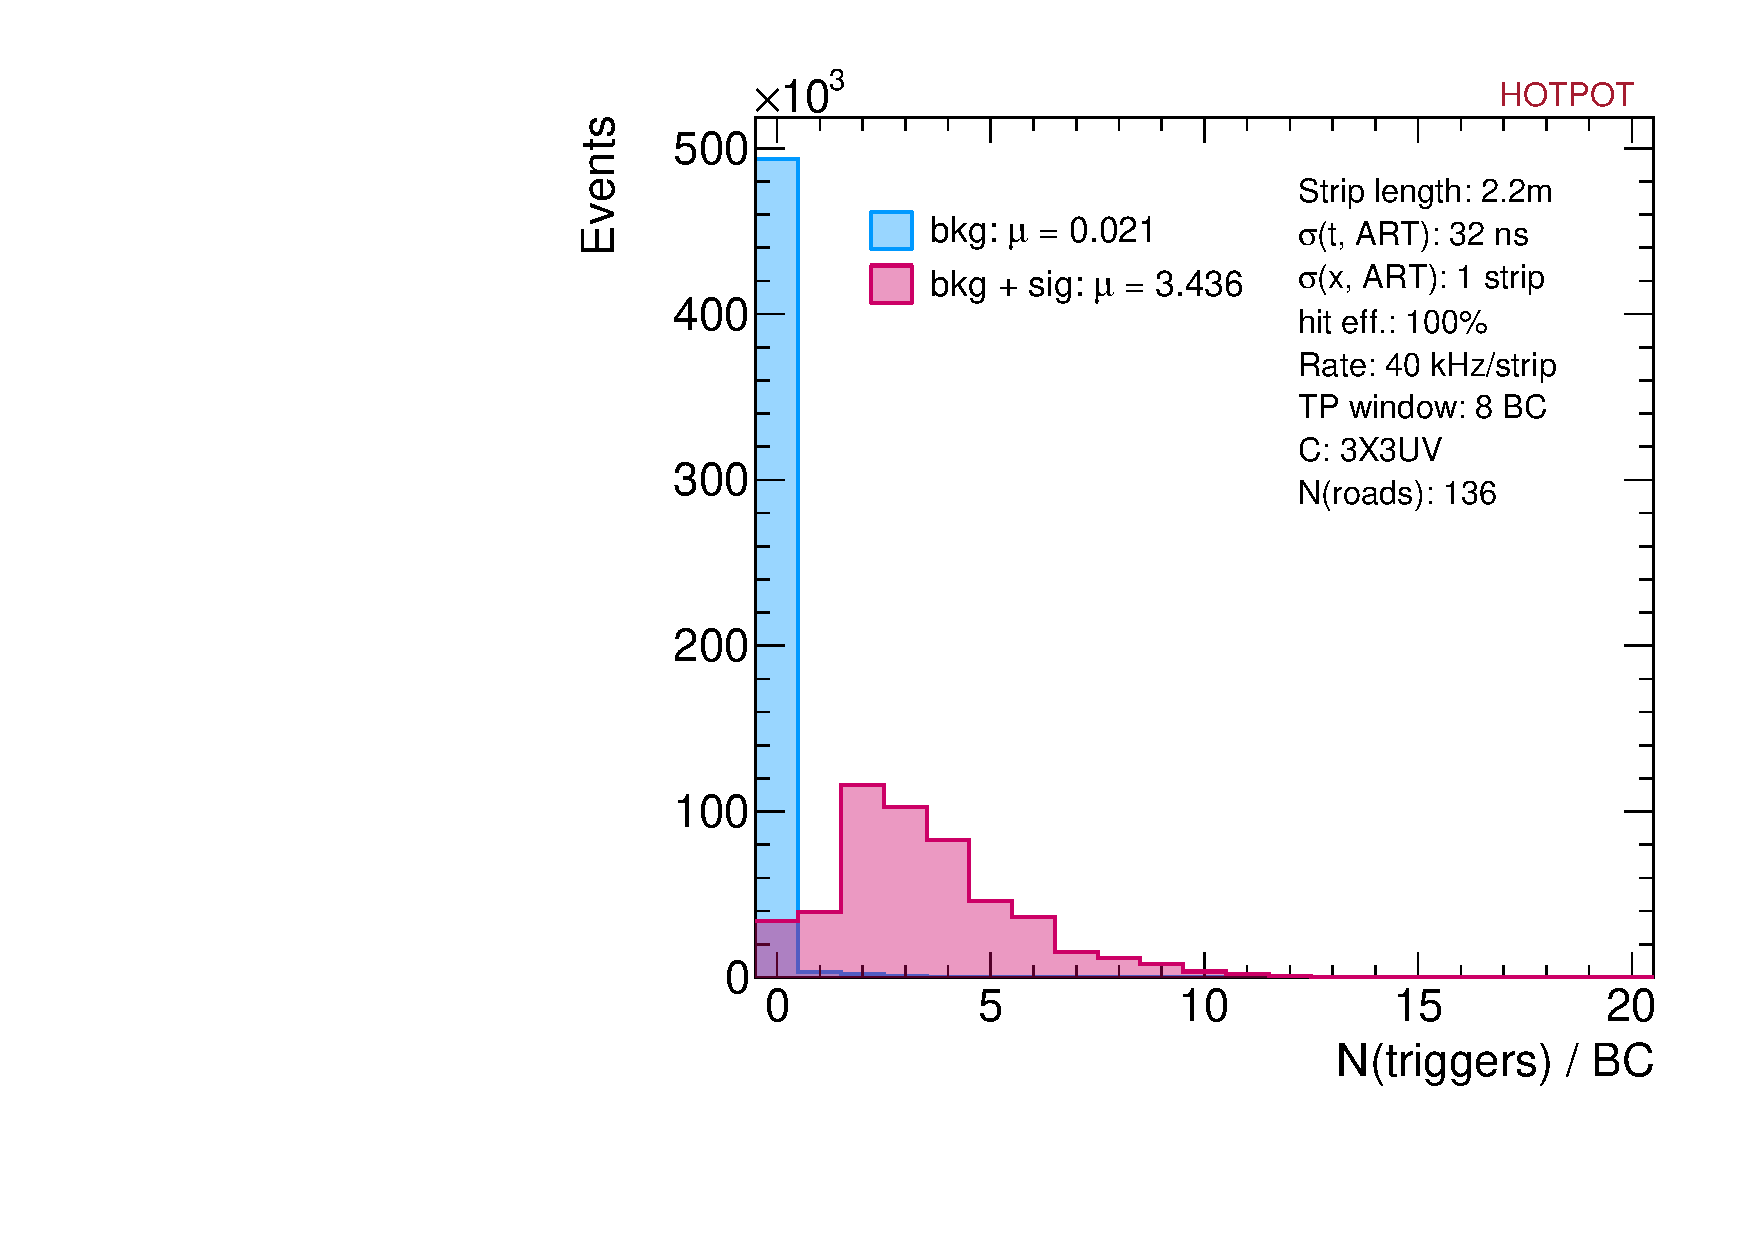
\includegraphics[width=0.48\textwidth]{figures/r136_ntrig_BC7.pdf}
  \end{center}
  \vspace{-10pt}
  \caption{Number of triggers found per BC for 0.5m long strips (left) and 2.2m long strips (right). The blue histogram represents the distribution if we only have uncorrelated background hits, and the pink histogram represents the distribution if we also add a muon track. For the pink histogram, since number of triggers in a given BC is dependent on the BC, we pick the BC when the first real muon ART hit is 8 BCs old.}
  \label{fig:ntrig}
\end{figure}
